\documentclass[sigconf]{acmart}

\usepackage{graphicx}
\usepackage{listings}

% Copyright
%\setcopyright{none}
%\setcopyright{acmcopyright}
%\setcopyright{acmlicensed}
\setcopyright{rightsretained}
%\setcopyright{usgov}
%\setcopyright{usgovmixed}
%\setcopyright{cagov}
%\setcopyright{cagovmixed}

% DOI
% \acmDOI{10.475/123_4}

% ISBN
% \acmISBN{123-4567-24-567/08/06}

%Conference
\acmConference[FDG 2019]{Foundation of Digital Games}{December 2018}{San Luis Obispo, California, USA}
% \acmYear{2019}
% \copyrightyear{2018}

\begin{document}
\title{Adaptive Procedural Narrative Generation in Text Games}

\author{Sean Mendonca}
\affiliation{%
  \institution{California Polytechnic State University}
  \streetaddress{1 Grand Ave}
  \city{San Luis Obispo}
  \state{California}
  \postcode{93405}
}
\email{smendon@calpoly.edu}

\author{Neal Nguyen}
\affiliation{%
  \institution{California Polytechnic State University}
  \streetaddress{1 Grand Ave}
  \city{San Luis Obispo}
  \state{California}
  \postcode{93405}
}
\email{nnguye57@calpoly.edu}

\renewcommand{\shortauthors}{Mendonca, Nguyen}

\begin{abstract}
This paper proposes a new approach for text based adventure generation AI and describes an implemented prototype for its core mechanisms. This prototype dynamically creates a narrative, without a pre-defined story tree, to provide an open world game experience to the player, where decisions made can affect the story. This prototype game remembers a user's personality from a static intro game and adapts to the user's personality as the player makes decisions. It keeps track of events that have occurred and picks the next major event based on that information. The game molds events on the fly, changing what happens, the characters that appear, and the possible options the player has.

This paper covers the current stages of the prototype for adaptive procedural narrative generation and the preliminary survey results, rating the success of the prototype game.
\end{abstract}

\maketitle

\section{Introduction} \label{Introduction}
Story is the backbone of many games. Traditionally, writers must spend a large amount of time putting a story together that makes the player feel like their decisions are impacting the game. This paper presents an automated approach that aims to reduce the amount of thought needed for new storylines by generating them on the fly and adapting them to a user's actions.

Currently, content generation through grammars is a solution that is applied to this problem. Grammars allow many potential options to be used at a given point. However, they have the major downside of being too static. They are unable to handle to handle variables during runtime, meaning they will not be able to act on history or provide unique options to different player types.

The most common approach in the modern game industry is the use of decisions trees. This approach is essentially hardcoded and will always have a set number of outcomes in the end. Using decision trees always requires a developer to manually write every potential story event, many of which are never seen by the majority of players. The cost to return ratio of this method forces developers to significantly limit either the depth or amount of storylines that can appear in their narrative.

\subsection{Our Contribution}
We aim to show, with a prototype in Renpy, that our text-based adventure generation model can create complex stories with many branches. Story events are decided on the fly as new events open and close based on what the player does. They can be written modularly and inserted, reducing the need for knowledge of the whole story, and making the addition of new events easier. Our player history system allows story events to be influenced by player personality and can be used to determine what options are available to a player at any given point.

\subsection{Paper Outline}
In the remainder of this paper, Section \ref{Background} covers previous works to narrative PCG (procedural content generation), Section \ref{Methods} covers how the prototype works at a high level, Section \ref{Results} shows user surveys results on the prototype, Section \ref{Discussion} analyzes these survey results to determine the viability of the prototype, and Section \ref{Conclusion} finishes with final thoughts and future works.

\section{Background} \label{Background}
Many existing games make use of a strong story focus, procedural narrative/quest generation, or some combination of both. Mainstream games at the time of this paper have yet to make use of procedural narrative generation but have used it in related elements such as quest generation. Procedural quest generation will dynamically assign players different tasks at different locations but usually does not feature a complex or detailed. The Elder Scrolls V: Skyrim \cite{skyrim} and Fallout 4 \cite{hernandez_2016} make extensive use of procedural quest generation which they call "Radiant Story" \cite{radiantAI}. The use of "Radiant Story" allows for potentially unlimited quests to be generated, with the downside of being extremely repetitive. Most Radiant Story quests involved unnamed generic NPCs, a simple goal (like kill all enemies at x location), and a limited set of dialogue lines. Many players have criticized certain radiant quests that were constantly triggered in Fallout 4.

\section{Methods} \label{Methods}
This Section covers our adaptive narrative PCG model in Subsection \ref{Adaptive PCG Model}. Then, Subsection \ref{Renpy} covers the visual novel engine Renpy, used for our game prototype. Finally, Subsection \ref{Karma History Prototype} presents the prototype and some screenshots from a playthrough.

\subsection{Adaptive PCG Model} \label{Adaptive PCG Model}
The game keeps track of event history and user personality in a global history object. A short pre-game segment is used to determine a player's starting personality and placement tags. Once a player completes the initial segment, the game will transition to different events based on pre/postconditions. Events form a directed graph where events that have post-conditions that are a subset of another event's pre-conditions from a link to that event. Events will randomly transition to any event in which their post-condition tags are a subset of another event's pre-condition tags. Player choices in an event sometimes add tags to that event's post-conditions before the possible edges are calculated.

\begin{figure*}[ht]
    \centering
    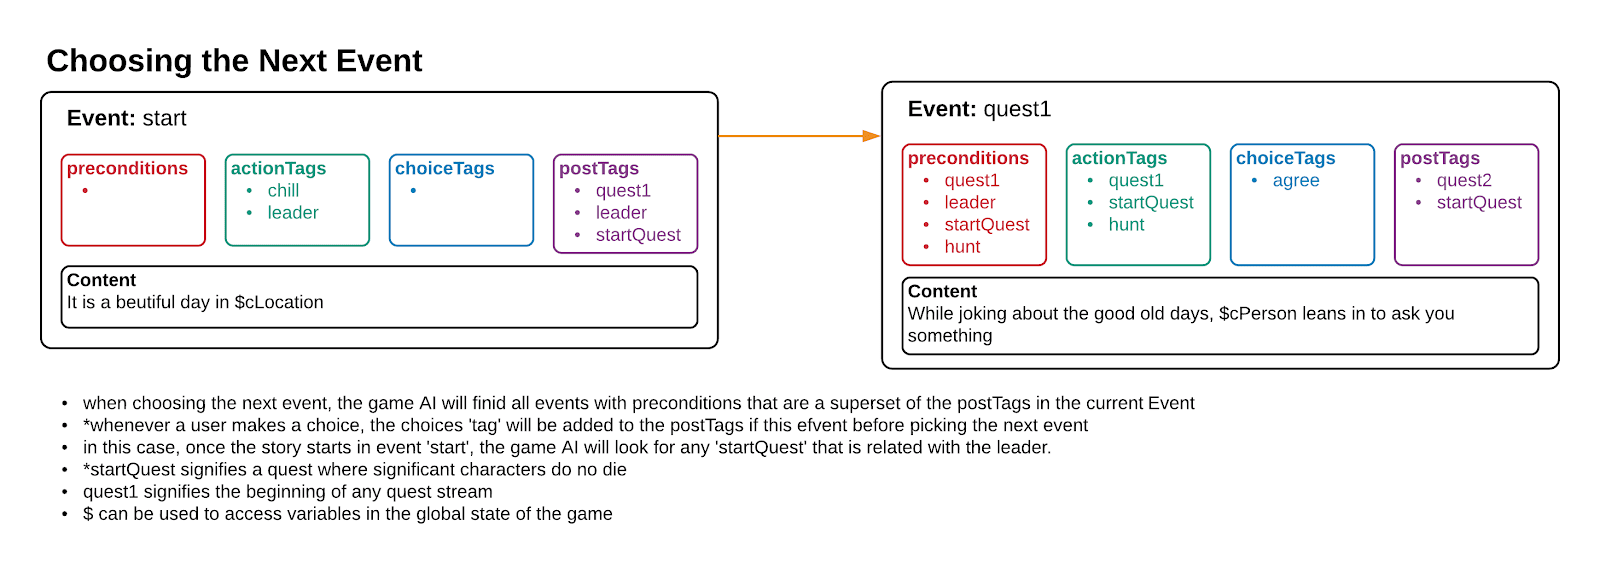
\includegraphics[width=\textwidth]{images/eventChoice.png}
    \caption{How an event is chosen}
    \label{fig:eventChoose}
\end{figure*}

Actions and NPCs (Non-Player Characters) appearing in events are determined with a tag system. The tag system can reference the global history structure to recall a previous choice or check if a condition has been met. Events contain separate tags to decide NPC actions and player choices. Not every event has to have either an NPC action or player choice; some include text to reflect on the outcome of the previous event/choice combination. NPC actions and player choices are chosen the same way as events, action and choice tags in an event must be a subset of the tags in the Action and Choice objects. An Event will randomly pick a suitable action and choice if possible. Actions also have a set of tags used to pick suitable NPCs for that action. 

\begin{figure*}[ht]
    \centering
    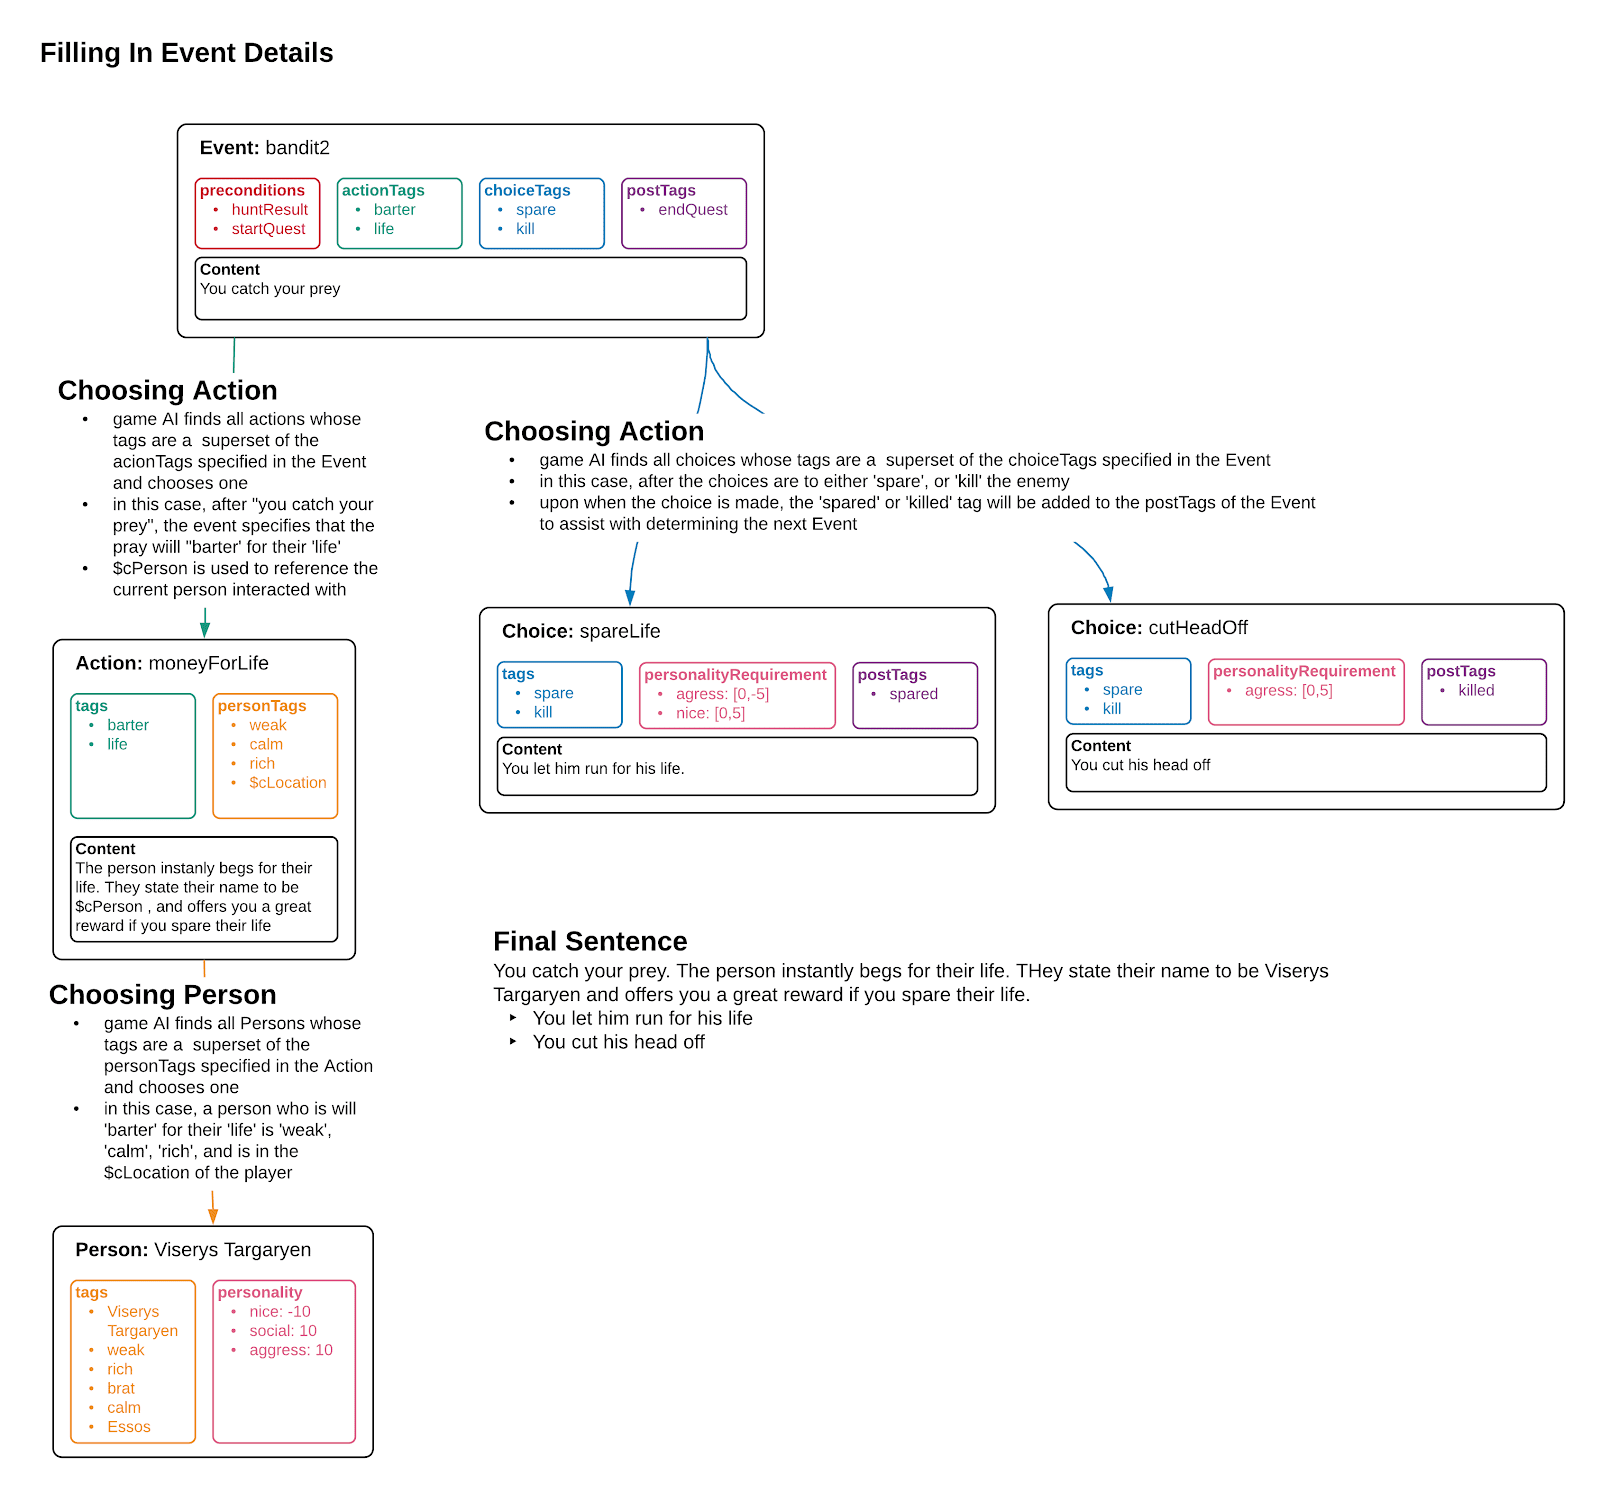
\includegraphics[width=\textwidth]{images/eventFill.png}
    \caption{How an event is broken down}
    \label{fig:eventFill}
\end{figure*}

NPC actions contain text describing what an NPC is doing. The presence of a set of person tags is to guarantee that a suitable NPC is picked for the action. For example, we never want a greedy character giving the player money for no reason. Every NPC character made for the game has unique personality values like the player, along with a set of tags that should specify their personality and background. The person chosen for an action is chosen the same way an action is, an NPC's tags must be a superset of the person tags in the Action object. An action is only suitable if at least one suitable NPC is found. The latest character chosen by an NPC action is saved to the global history, so it is not always necessary to generate a new action/character tag at every event. This allows developers to guarantee specific event lines when desired, allowing for scenes spanning several conversation points.

Choice objects contain text specifying what the player is doing in that choice, tags to be picked by an event, a personality requirement in order to be used by a player, a value to modify the player's personality if chosen, and any amount of post-tags to added to the event's post tags if chosen. The optional post tags are used to mark significant decisions, such as the death of a major character. These post tags can also be used to alter the global game state by adding/removing tags from NPC characters. This is essential to ensure that events transition appropriately based on choices.

There are many possible combinations of actions and people when the two objects are written as intended. This makes the tag system paramount to the results of narrative generation in Karma History. We already make use of two special tags in the game. The \$ tag retrieves a specified variable from the global history; this is used to fill in names, actions, and choices from previous events. The \# is used for a pre-condition global history check by events. It was unfeasible to grow the tags passed by an event's continuously, so we use \# tags to block progression to points of the story that do not make sense given the current global state. \#tags are removed from an event's pre-condition once the global condition they specify is met.

\subsection{Renpy} \label{Renpy}
We used Renpy \cite{renpy} to implement a prototype for this model. Renpy is a visual novel engine that displays an image in the background and text as shown in Figure \ref{fig:customLannister}. The text field can present choices, text entry fields, or just strings. It is built on top of Python \cite{python} allowing for embedded python scripts within the Renpy scripting language.

Renpy was chosen for this project because it was lightweight, simple, and provides the basic features for a narrative game. Its ability to include embedded Python was the biggest factor in creating a quick prototype. Python is a common language we both already knew with quick setup time. Learning a new system such as Unity \cite{unity} was desired, but would take too long to learn.

\subsection{Karma History Prototype} \label{Karma History Prototype}
To prototype our Adaptive PCG model with Renpy, we created a game called Karma History, based on Game of Thrones \cite{got}. This prototype is a proof of concept for our model through the surveys in section \ref{Results}. Figures \ref{fig:menu} to \ref{fig:customLannister} show Karma History at different points in the game. 

\begin{figure}[ht]
    \centering
    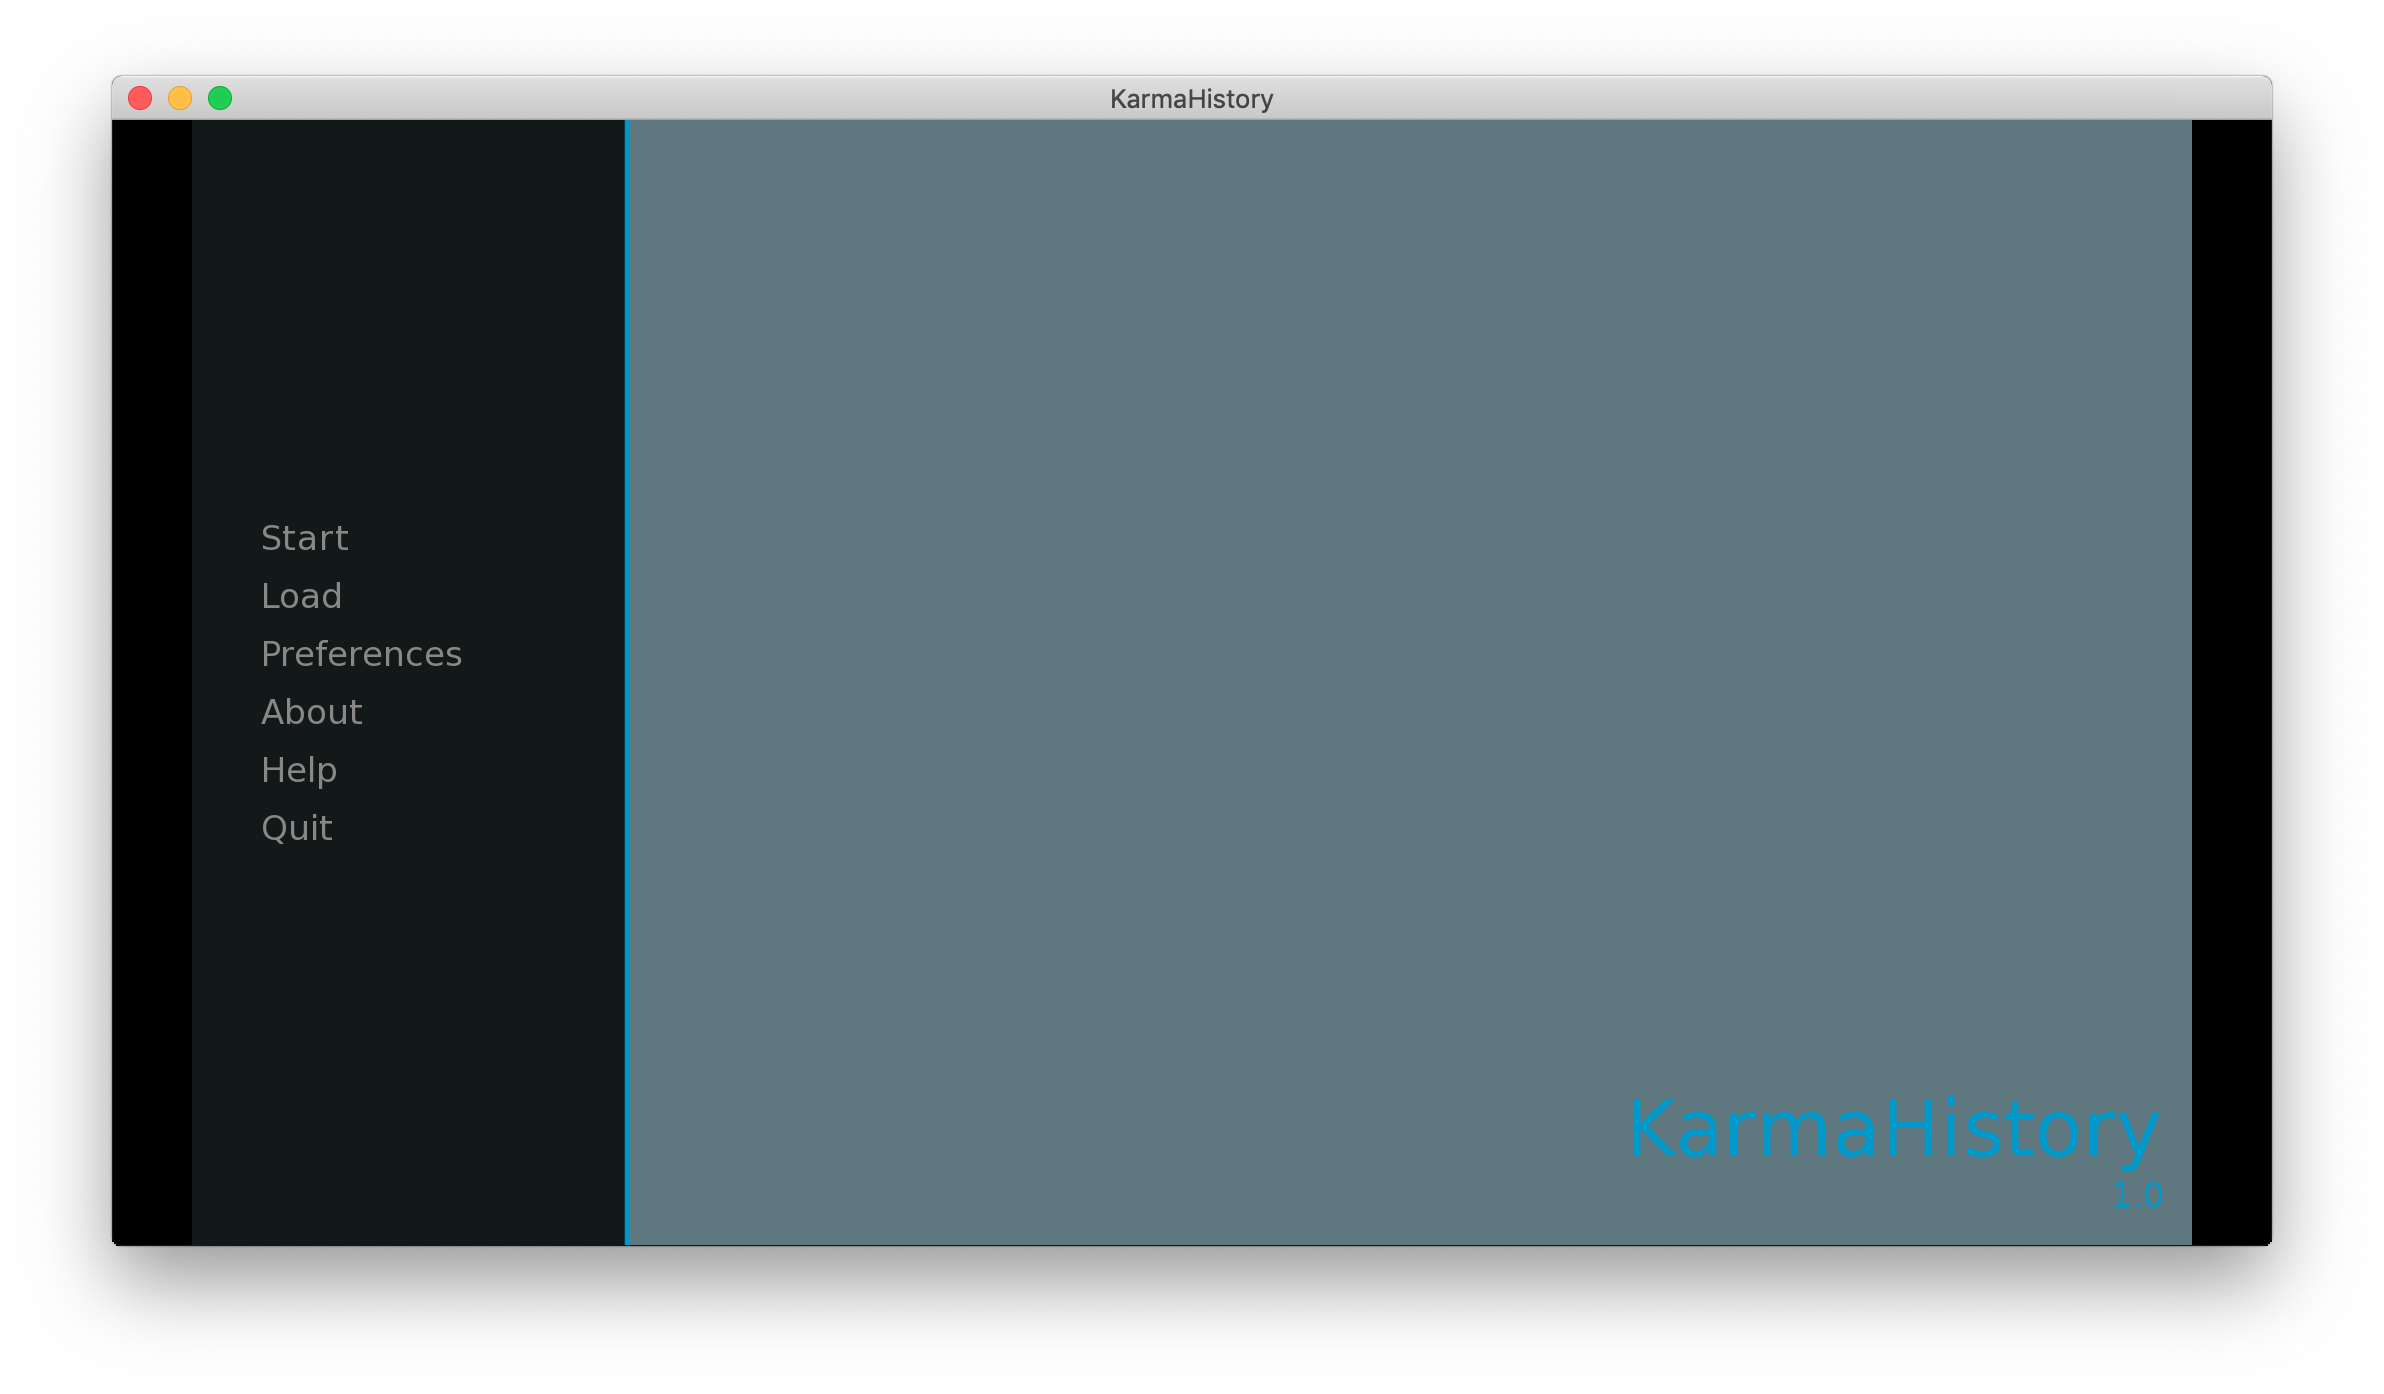
\includegraphics[width=0.4\textwidth]{images/menu.png}
    \caption{Start menu for prototype game.}
    \label{fig:menu}
\end{figure}

\begin{figure}[ht]
    \centering
    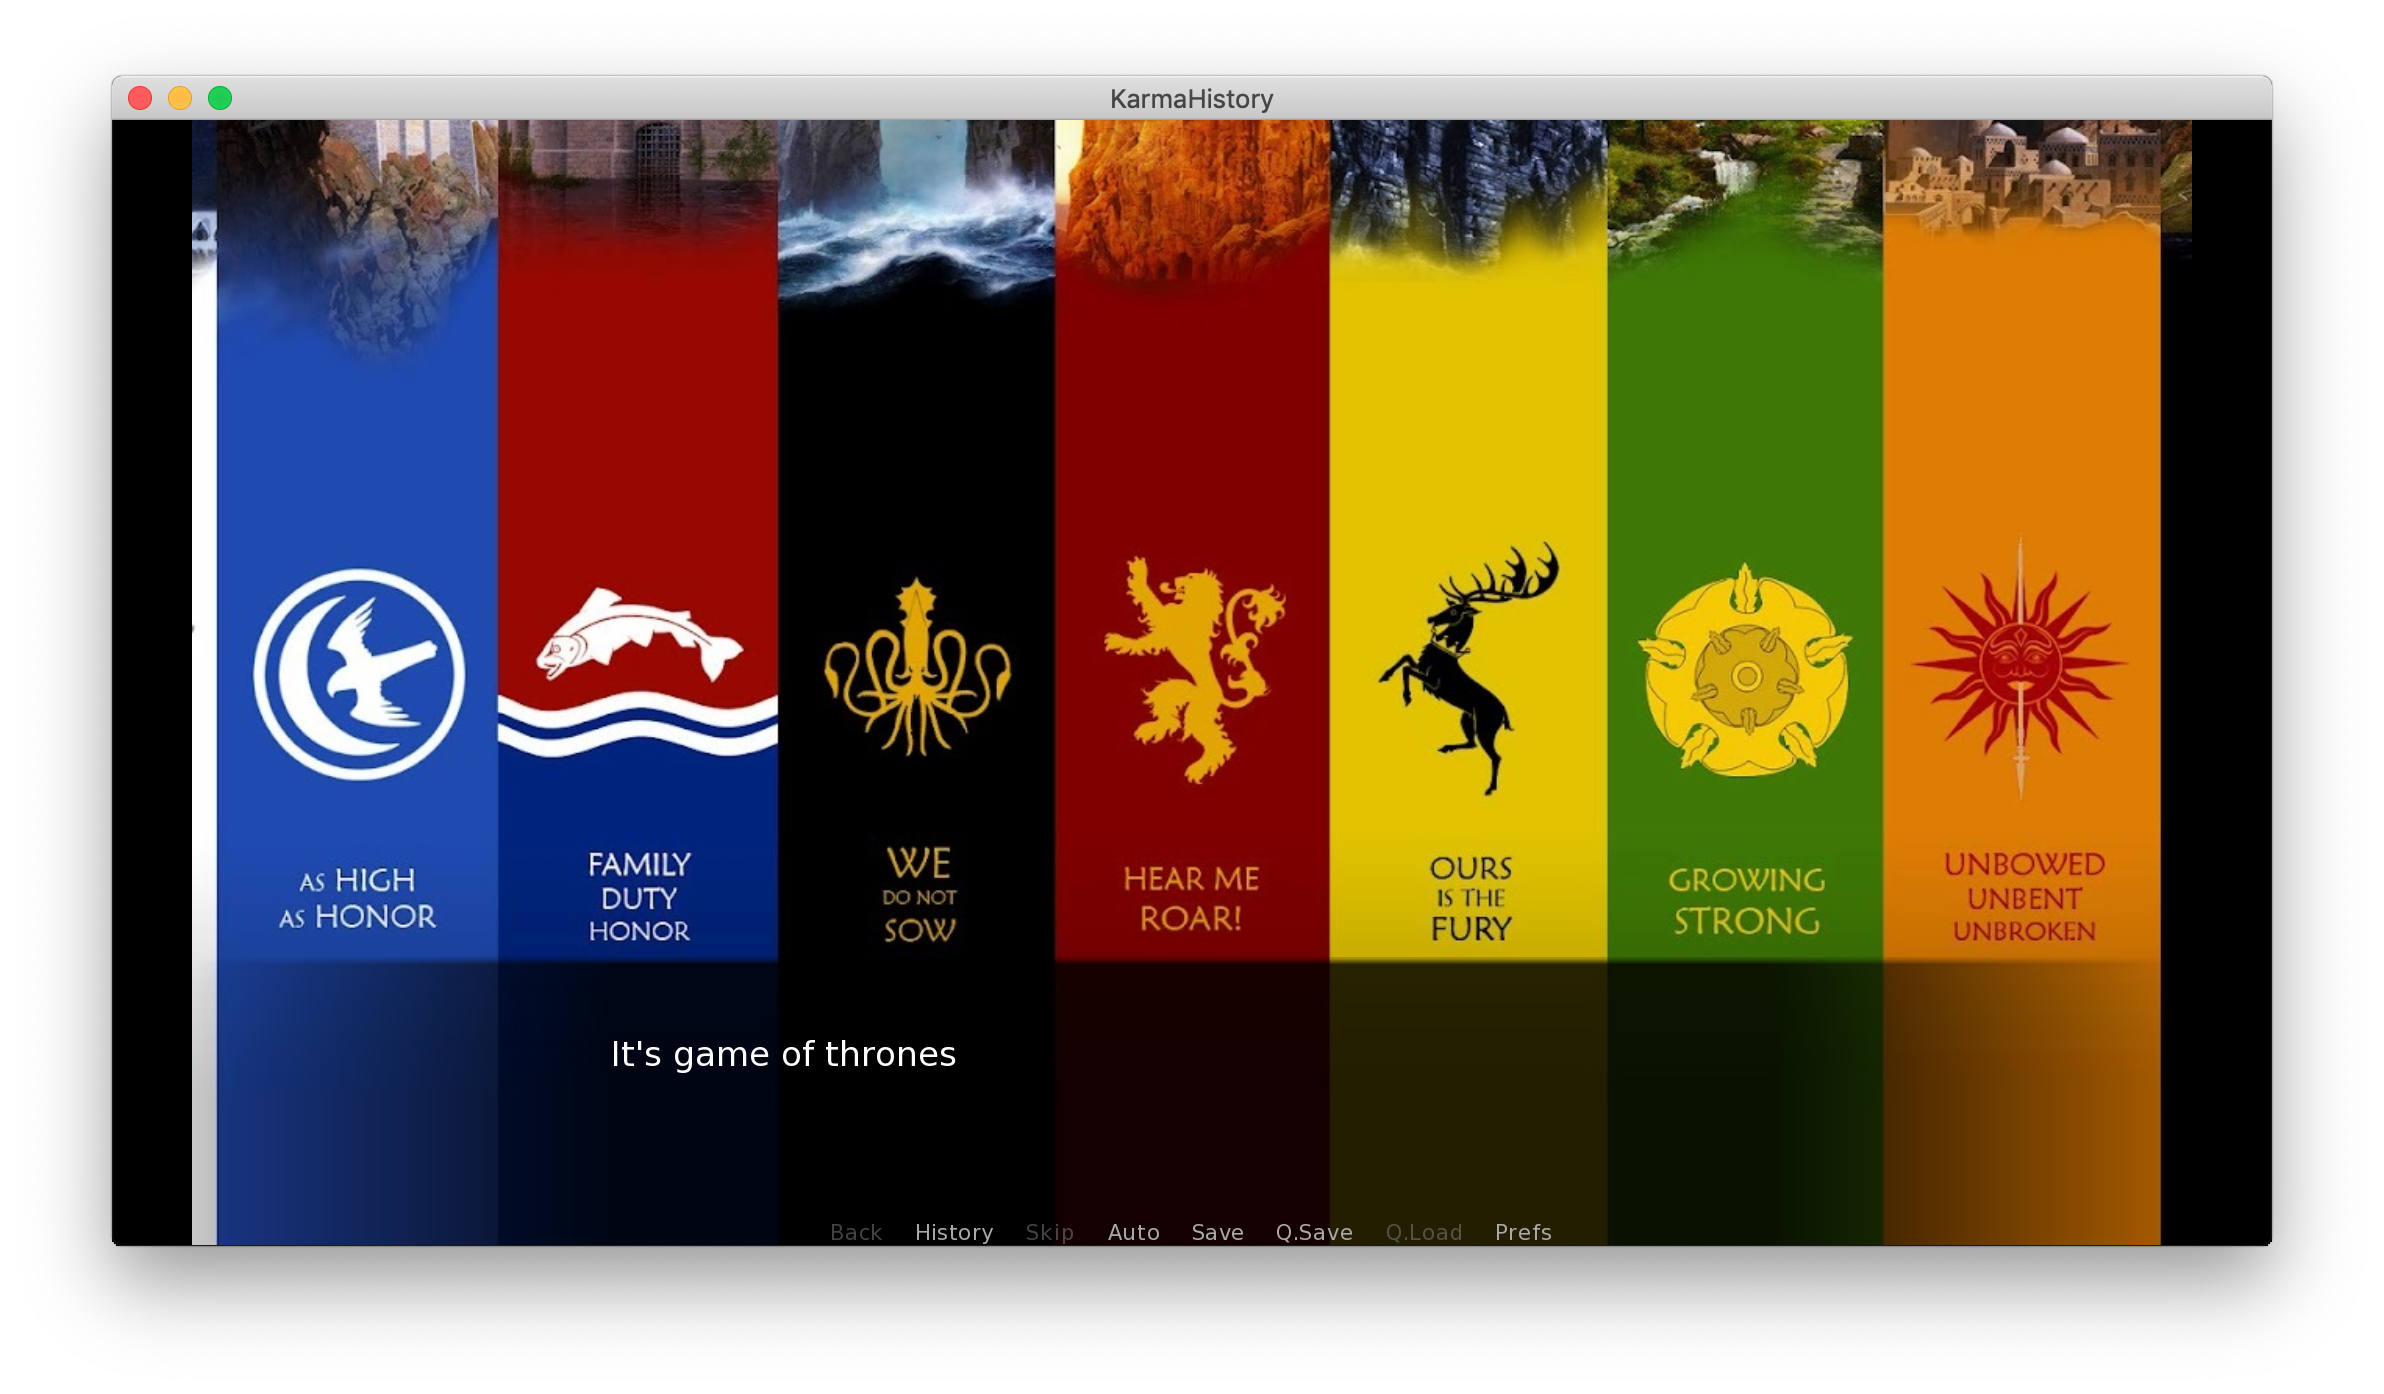
\includegraphics[width=0.4\textwidth]{images/gameStart.png}
    \caption{Opening screen for prototype game.}
    \label{fig:gameStart}
\end{figure}

\begin{figure}[ht]
    \centering
    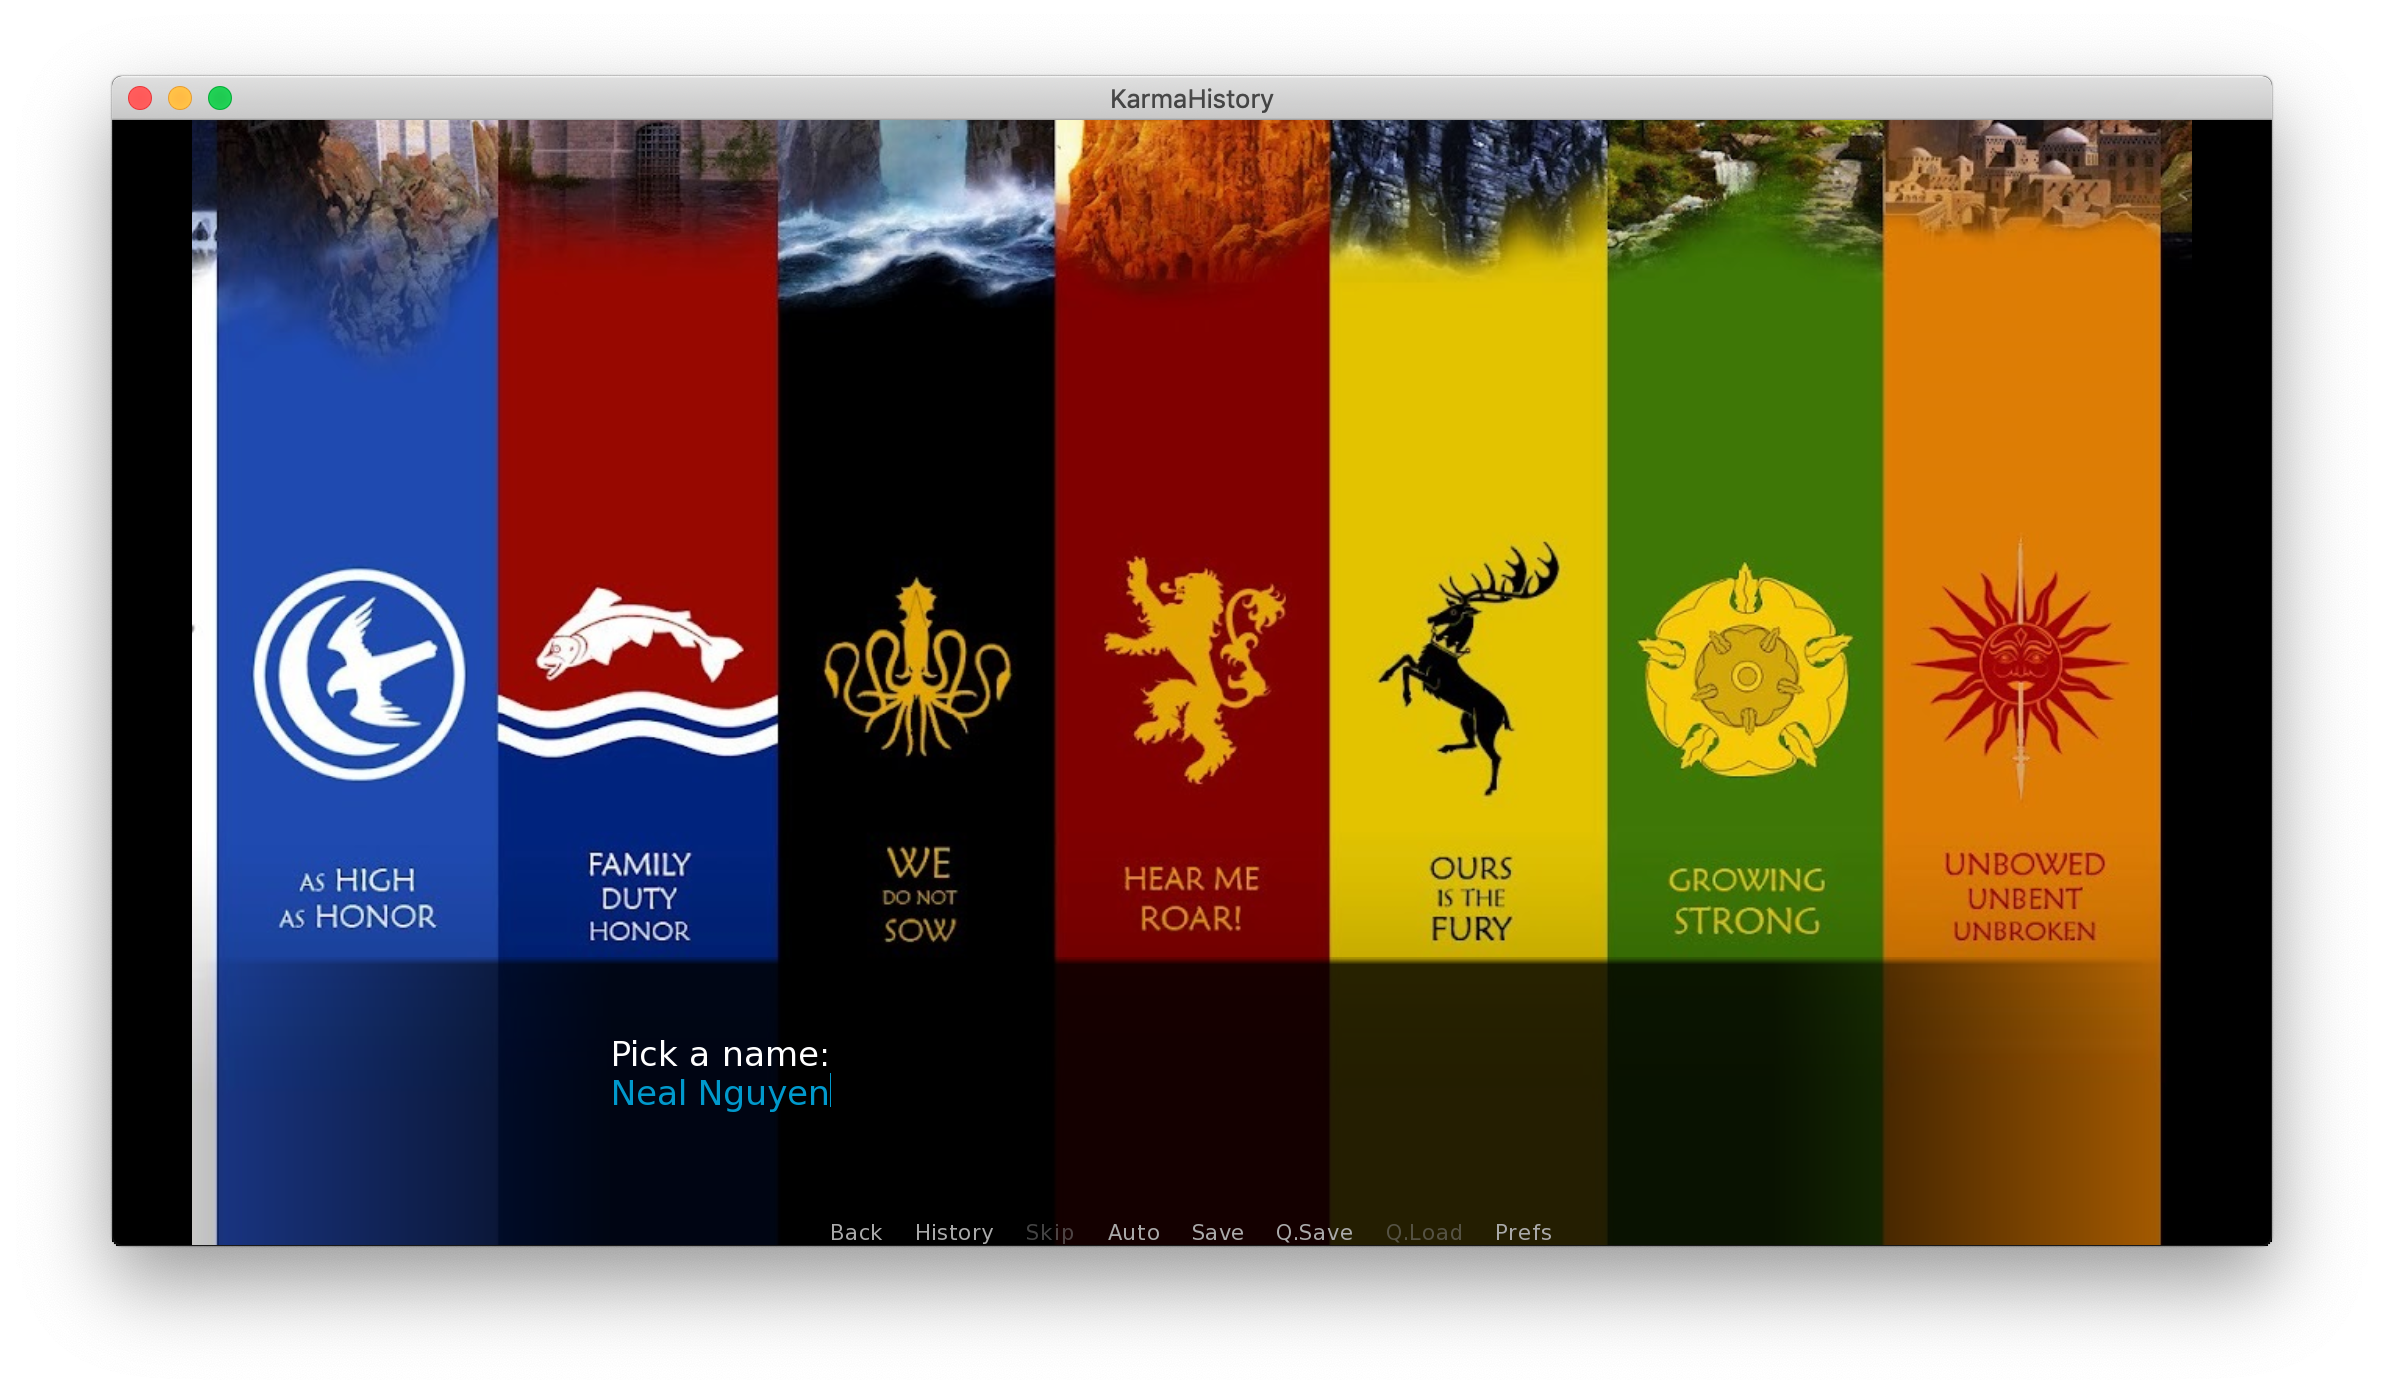
\includegraphics[width=0.4\textwidth]{images/chooseName.png}
    \caption{Entering player name for prototype game.}
    \label{fig:chooseName}
\end{figure}

\begin{figure}[ht]
    \centering
    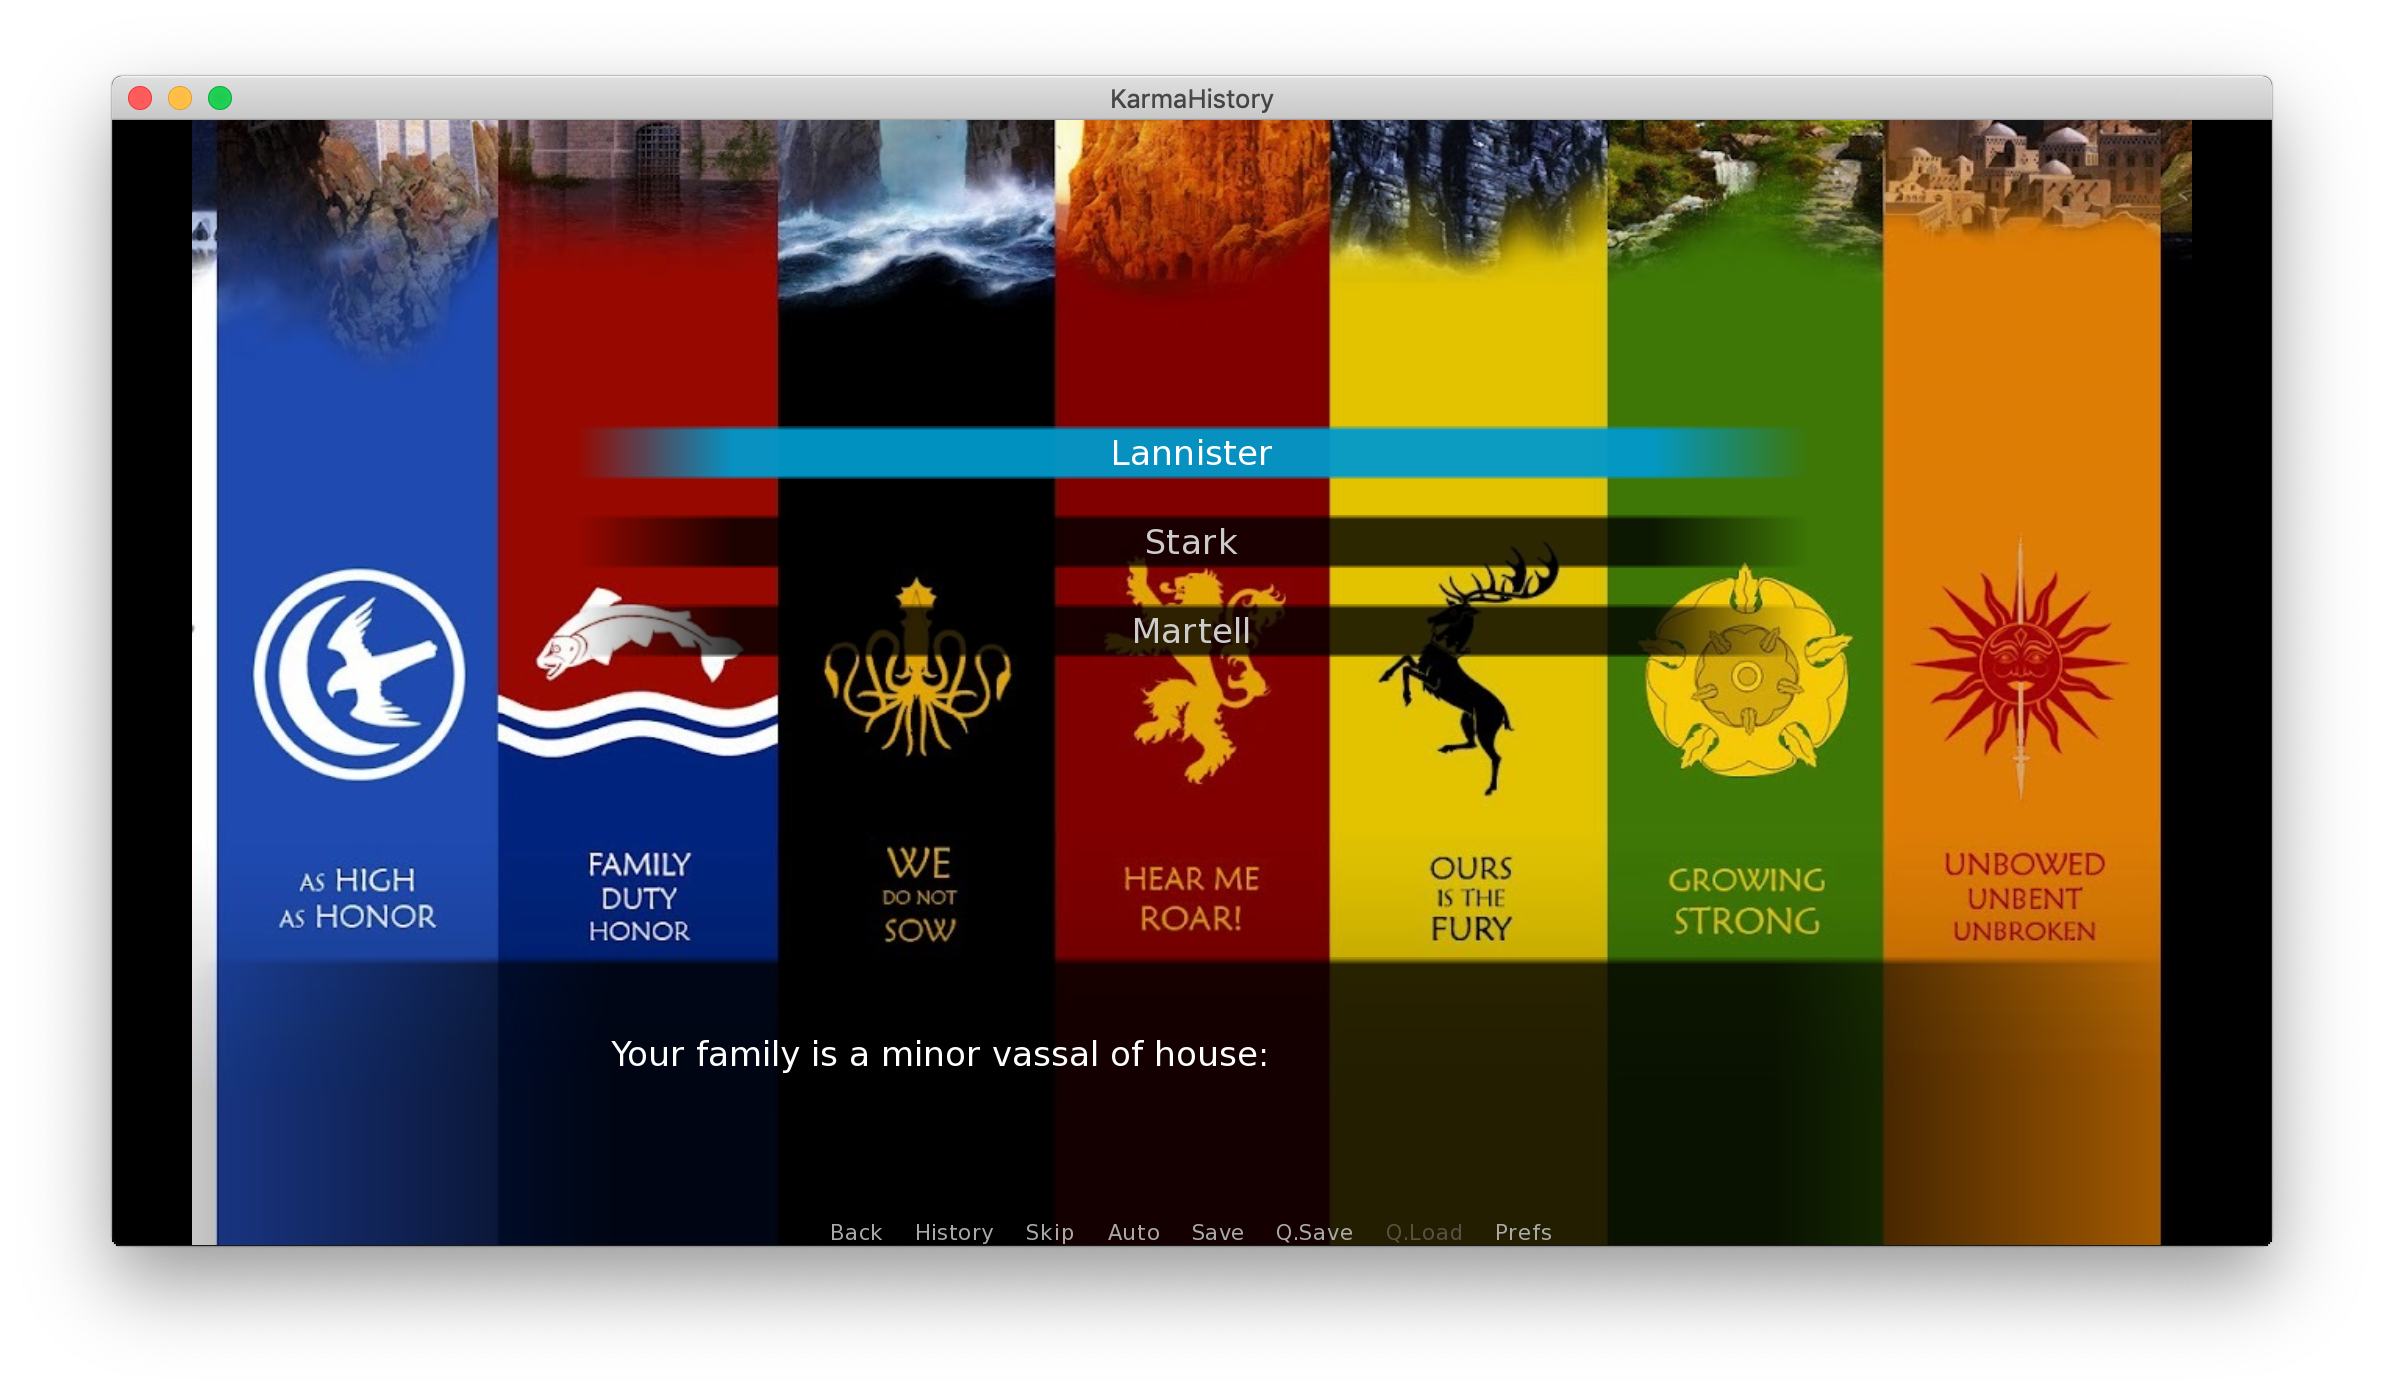
\includegraphics[width=0.4\textwidth]{images/chooseHouse.png}
    \caption{Choosing player house alliance for prototype game.}
    \label{fig:chooseHouse}
\end{figure}

\begin{figure}[ht]
    \centering
    \includegraphics[width=0.4\textwidth]{images/preGame.png}
    \caption{Static pregame at the beginning of each play through to calibrate player personality.}
    \label{fig:preGame}
\end{figure}

\begin{figure}[ht]
    \centering
    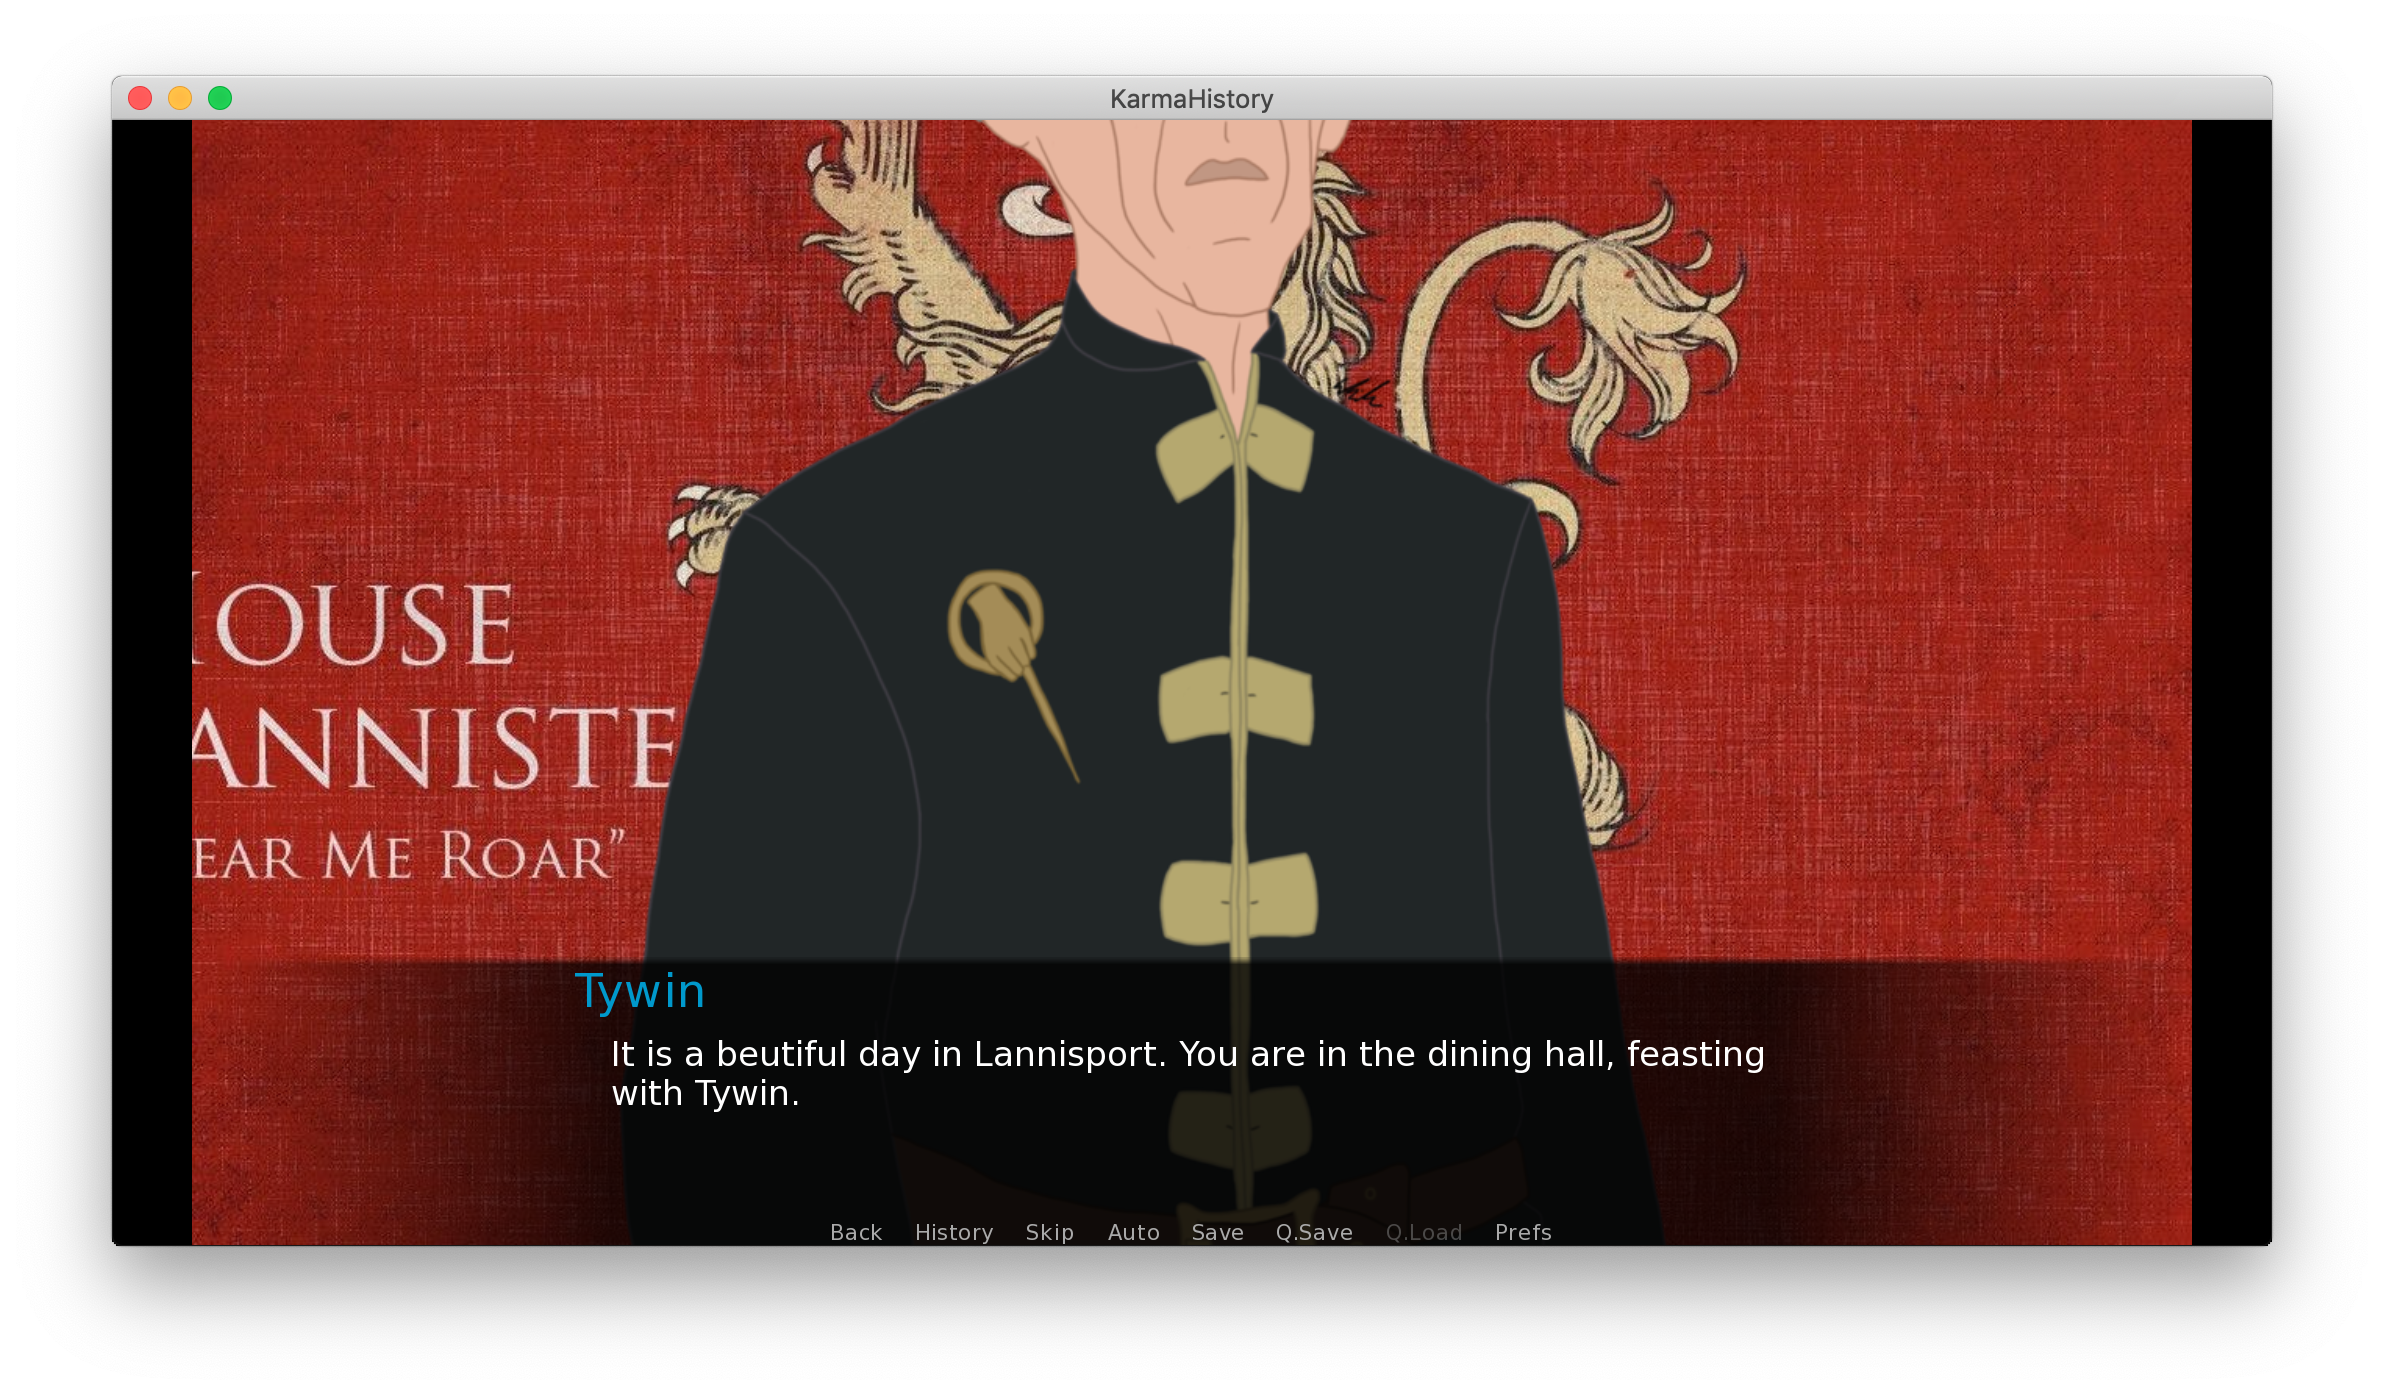
\includegraphics[width=0.4\textwidth]{images/customLannister.png}
    \caption{Start of adaptive PCG prototype pregame after house is chosen and personality is calibrated}
    \label{fig:customLannister}
\end{figure}
\section{Results} \label{Results}
At the time of this paper, only a brief survey has been conducted on a very early prototype of Karma History. We were only able to test an early prototype of our game which had about 5 minutes of content. Since we focused on generating different content both randomly and based on the player's choices we had each player play through our prototype twice. We noticed that players would spend a significant amount of time on the pre-game segment. Most players would pick the "good guys" faction of the world we represented in our prototype. The next phase would have a different location and character depending on the faction they picked. The next events could have varying numbers of choices for the player to pick depending on their choices in the earlier segments. This might not have been obvious to the players unless they were paying careful attention during their next playthrough. Unfortunately, a large portion of our testers experienced bugs or crashes that affected the overall quality of the session.
\par
After playing the game, each player was asked to take a short survey. The survey contained some short answer sections as well as sections asking a player to rate a value from 1 to 5. The key features we wanted each user to rate was, "Is the game creative?", "Does the generated story make sense?", and "Was the generated story varied?".

\begin{figure}[ht]
    \centering
    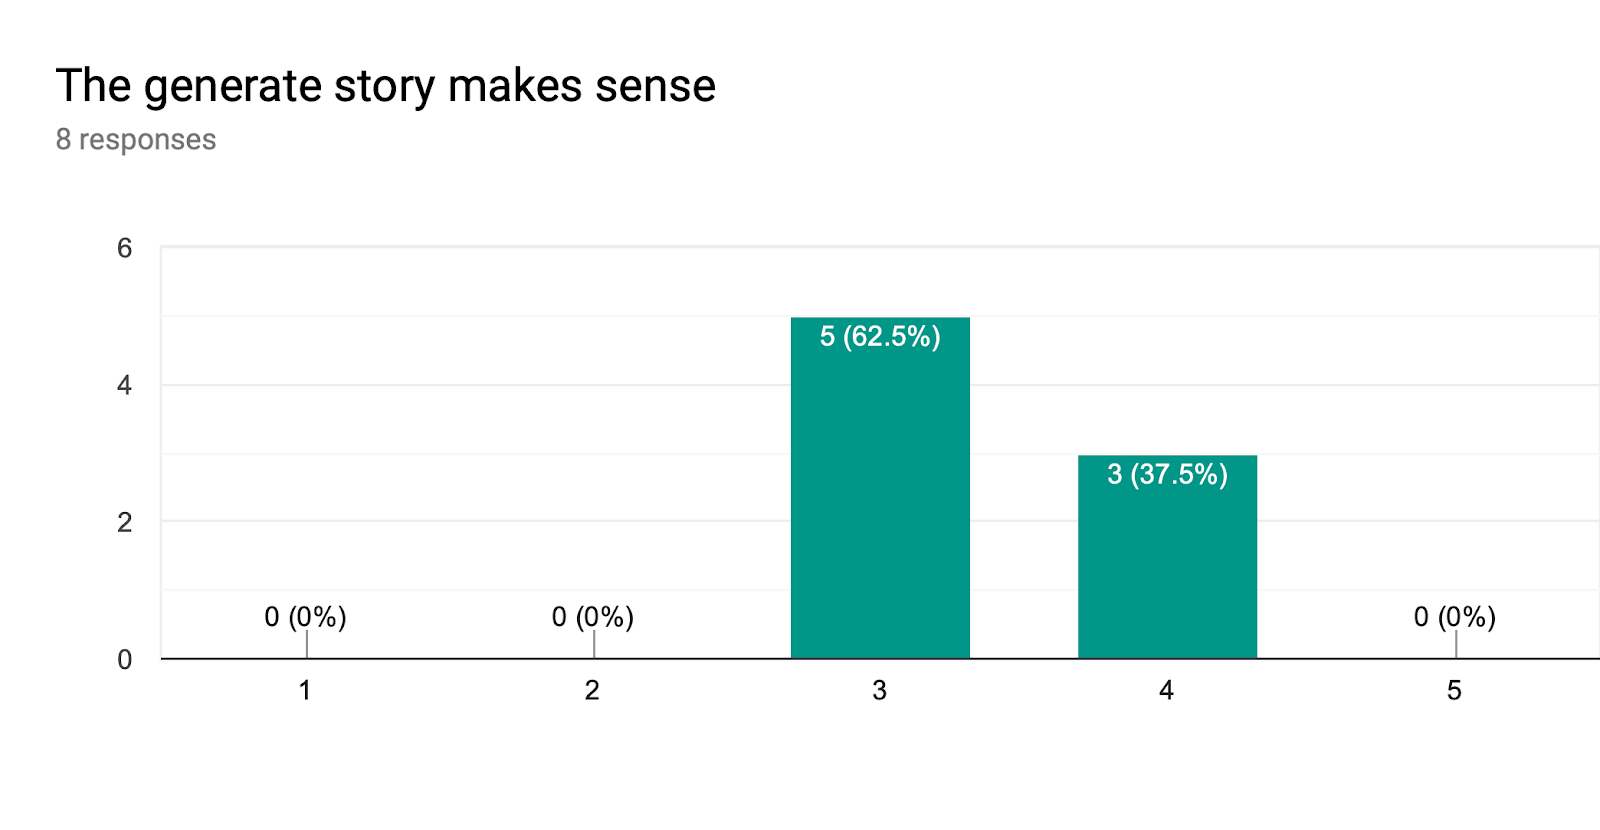
\includegraphics[width=0.3\textwidth]{images/s1.png}
    \caption{Survey: makes sense}
    \label{fig:s1}
\end{figure}

The results to "Is the game creative" were slightly positive but mostly neutral. As seen in \ref{fig:s2} the majority of users answered with either a 3 or 4. The results for "Does the generated story make sense?" \ref{fig:s1} and "Was the generated story varied" \ref{fig:s3} were similar. The results hint that our prototype showed some of these aspects, but not to a strong degree.

\begin{figure}[ht]
    \centering
    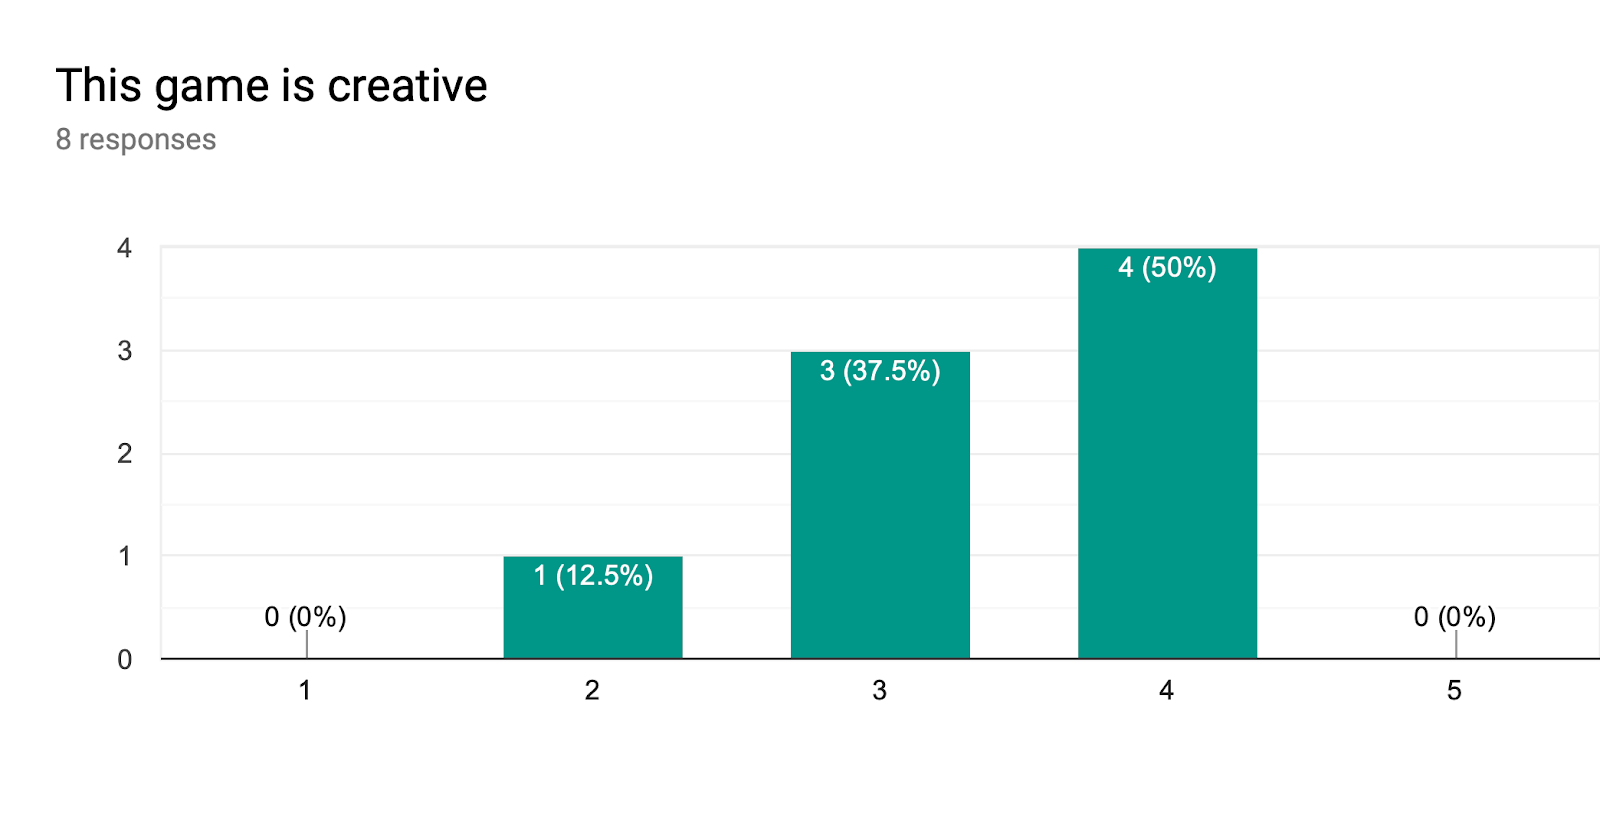
\includegraphics[width=0.3\textwidth]{images/s2.png}
    \caption{survey: is creative}
    \label{fig:s2}
\end{figure}

\begin{figure}[ht]
    \centering
    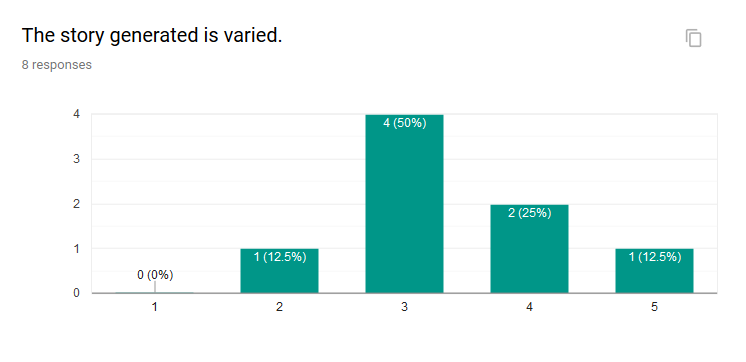
\includegraphics[width=0.3\textwidth]{images/s3.png}
    \caption{survey: story generation is varied}
    \label{fig:s3}
\end{figure}
\section{Discussion} \label{Discussion}
Given the preliminary results from \ref{Results} as well as our own experience with the project, we believe there are some issues to address with our current implementation. We found that it currently takes a lot of writing and tagging to keep the story consistent and that the system is difficult to debug due to the random nature of the model. Minor mistakes with tagging lead to undefined behavior or crashes. Our system may be procedural in design, but it still requires a developer to put a significant amount of time into writing characters and potential storylines. We did not have enough time to reach the level of detail we hoped in our demo, and believe additional writing/debugging is needed to showcase the strengths of our model.

The random nature of the system could lead to repetitive behavior. We designed a fight scene that could last a variable number of events, and many users became convinced they were stuck in a loop and tried the "run away" option. The obvious solution to this would be to prevent specific events from occurring again, however, doing this eliminates generic events that can be used in a number of different places. For example, it would make the developer have to write a different death scene for every possible character; this would effectively reduce our model to a random decision tree. Discussion on how to resolve this narrative problem is ongoing.

Renpy was an easy platform to test our ideas on, but many of the engine's features are not adapted for the random nature of PCG. The game is designed to support a GOTO style of event transition which is not supportive of randomly and dynamically changing the story during runtime. Due to this, core Renpy features such as saving and the back button do not function as intended. Renpy provides an easy visual framework to test our ideas on, but further testing would need to be done to see if the engine can fully support PCG.

\section{Conclusion} \label{Conclusion}
Karma History can generate different narrative trees based on user decisions but can be prone to the repetition that many PCG games face. It can dynamically construct a narrative out of potential events, actions that can occur in them, and NPC characters that fit the requirements of the potential actions. The flexible tagging system allows developers to guarantee details and a linear progression when needed, but also allows the story to develop dynamically. The system is still in need of refining but overall shows potential.

\section{Future Work}
We hope to increase the amount of story detail now that our model is functional. Our priority is to add more personality to interactions so that the player feels that their decisions matter. We are investigating what would be the easiest approach to make NPC dialogue dependant on a player's personality and choices. The use of a contextual grammar is also being explored for this purpose; global history values could be passed to determine appropriate gender pronouns and verbs for objects. More events are also needed for our prototype; the current number only displays three potential separate event chains even though the actual content in those events could vary a good amount.

\bibliographystyle{ACM-Reference-Format}
\bibliography{sources}

%Show Renpy Code Here

\end{document}
